\section {Results}
\label{results}

\subsection {Analysis} 
%Since $H_{1}$ concerns the mean count of xyz for each word, a one-tailed Student's Independent \textit{t}-test will be used here to determine whether the mean count of xyz for nouns are statistically significantly greater than those for adjectivs.  The threshold for significance adopted here is $0.01$.  

\subsection{Genetic Algorithm Number}%for appendix
We used a 3-level for-loop structure to vary the parameters of the genetic alignment algorithm to produce differing alignment algorithms---each one having its own preferences. 

\subsubsection{Settings}
Our 3-level for-loop having 2 settings for word order (forward/reverse) and 4 settings for synset strictness (off/1/2/3), subsequently, results in 8 algorithms. Figures xyz %~\ref{best settings}
shows the settings used for each of them.%to achieve the lowest error for each imitation type.


\begin{tabular} {|l | c | c |}
	\hline	\textbf{Algorithm Number} & \textbf{Word Order} & \textbf{Synset strictness}\\
	\hline	1	&	2	&	3	\\
	\hline	2	&	2	&	3	\\
	\hline	3	&	2	&	3	\\
	\hline	4	&	2	&	3	\\
	\hline	5	&	2	&	3	\\
	\hline	6	&	2	&	3	\\
	\hline	7	&	2	&	3	\\
	\hline	8	&	2	&	3	\\ \hline
\end{tabular}

\subsection{Overall Error}
Figure xyz %~\ref{algorithmsTotalError} 
shows the overall error for version of the genetic algorithm. The best overall was algorithm 1 with an RMSE of $184.89$ while the worst had an RMSE of $xyz$.
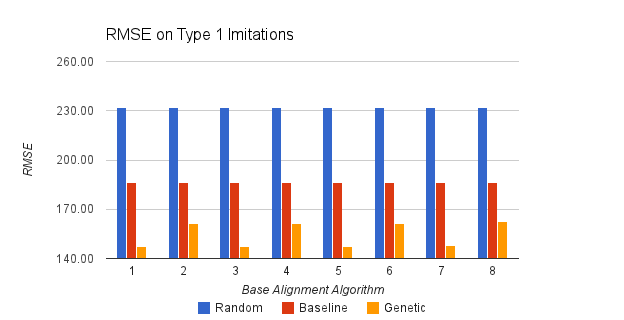
\includegraphics[width=16cm]{images/chart1.png}

\subsection{Error By Imitation Class}
Figures xyz-xyz %~\ref{alg1totalerror}-~\ref{alg8totalerror} 
demonstrate that the various versions of genetic alignment behave differently. Their differing preferences causes them to sometimes be more adept for certain citation classes. The best genetic algorithm for each class is given below:


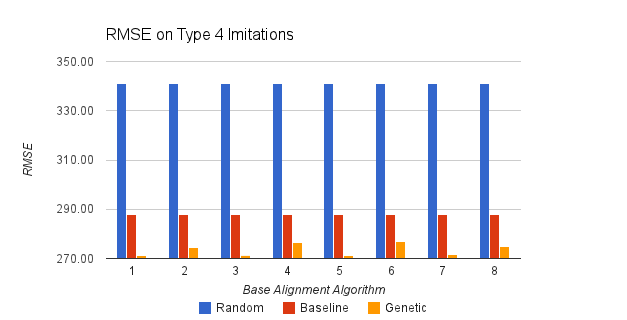
\includegraphics[width=16cm]{images/chart2.png}
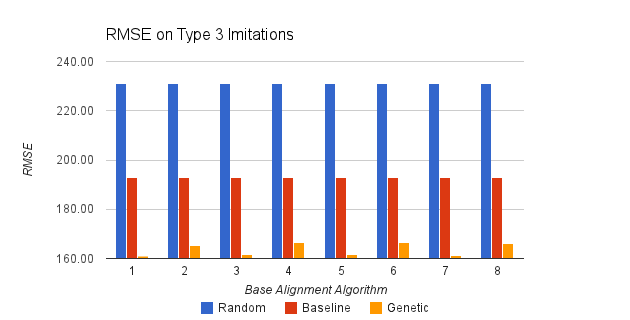
\includegraphics[width=16cm]{images/chart3.png}
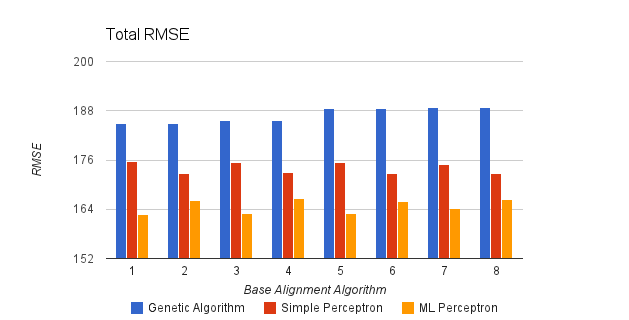
\includegraphics[width=16cm]{images/chart4.png}
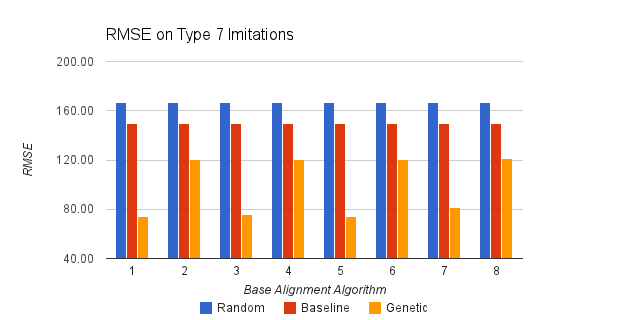
\includegraphics[width=16cm]{images/chart5.png}
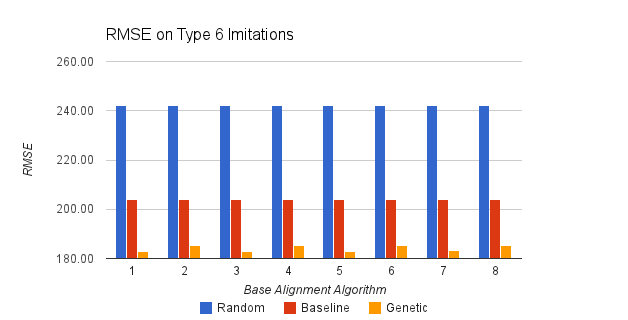
\includegraphics[width=16cm]{images/chart6.png}
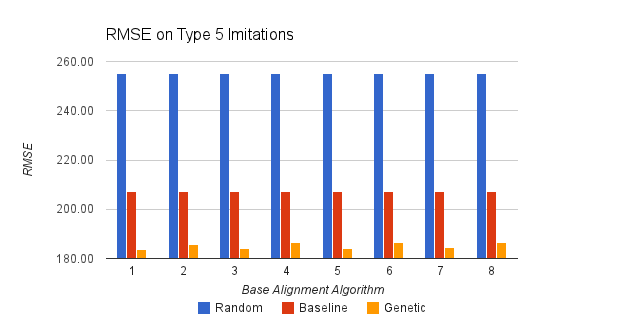
\includegraphics[width=16cm]{images/chart7.png}
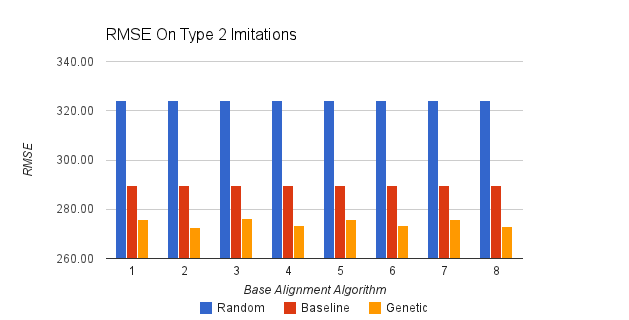
\includegraphics[width=16cm]{images/chart8.png}

%\subsection{Best in Each Category}
%Figures xyz %~\ref{theoreticalCombinedError} 
%shows the lowest error achieved for each imitation type. 
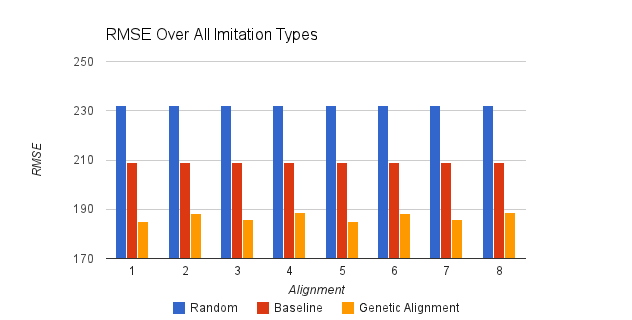
\includegraphics[width=16cm]{images/chart9.png}
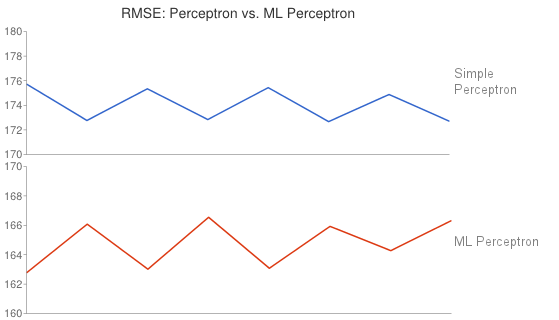
\includegraphics[width=12cm]{images/chart10.png}


\subsection{BP-trained ANN Performance}
(xyz fill this in)

%%%%%%%%%%%%%%%%%%%%%%%%%%%%%%%%%%%%
%sample helps from previous research
%%%%%%%%%%%%%%%%%%%%%%%%%%%%%%%%%%%%

%Tables~\ref{tab:all_adjective}, \ref{tab:all_noun} show the normalized responses and total counts for each set of xyz while Table~\ref{tab:all_group_stats} shows the group statistics for the two groups.


%\begin{table}
	\begin{center}
		\begin{tabular}{|c|c|c|c|c|} \hline
			\textit{HOT} & \textit{BLACK} & \textit{TALL} & \textit{LARGE} & \textit{UGLY} \\ \hline \hline
			cold	&	white	&	short	&	small	&	pretty		\\
			cold	&	white	&	short	&	small	&	beautiful		\\
			cold	&	white	&	short	&	tiny	&	beautiful		\\
			cold	&	white	&	short	&	small	&	beautiful		\\
			not hot	&	not black	&	not tall	&	not large	&	not ugly		\\
			cold	&	white	&	short	&	small	&	pretty		\\
			cold	&	light	&	short	&	petite	&	pleasing		\\
			cold	&	white	&	short	&	small	&	beautiful		\\
			frigid	&	white	&	short	&	miniscule	&	breathtaking		\\
			ugly	&	white	&	short	&	small	&	pretty		\\
			cold	&	white	&	short	&	small	&	pretty		\\
			cold	&	white	&	short	&	small	&	pretty		\\
			cold	&	white	&	short	&	small	&	beautiful		\\
			cold	&	white	&	short	&	small	&	pretty		\\
			cold	&	white	&	short	&	small	&	beautiful		\\
			cold	&	white	&	short	&	small	&	pretty		\\
			cold	&	white	&	short	&	small	&	pretty		\\
			cold	&	white	&	short	&	small	&	beautiful		\\
			cold	&	white	&	short	&	small	&	Beauty 		\\
			cold	&	white	&	short	&	small	&	pretty		\\
			cold	&	white	&	short	&	small	&	beautiful		\\
			cold	&	white	&	short	&	small	&	pretty		\\
			cold	&	white	&	short	&	small	&	beautiful		\\
			cold	&	N/A	&	N/A	&	N/A	&	beautiful		\\
			cold	&	white	&	short	&	small	&	beautiful		\\
			cold	&	mirrored	&	short	&	small	&	beautiful		\\
			freezing	&	N/A	&	N/A	&	insignificant	&	N/A		\\
			cold	&	white	&	short	&	small	&	beautiful		\\
			cold	&	light	&	diminutive	&	petite	&	exquisite		\\
			cold	&	white	&	short	&	small	&	beautiful		\\
			cold	&	white	&	short	&	small	&	pretty		\\
			cold	&	white	&	short/small	&	small	&	pretty		\\
			%cold	&	white	&	short	&	small	&	beautiful		\\
			%cold	&	white	&	short	&	small	&	beautiful		\\
			cold	&	white	&	short	&	small	&	pretty		\\ \hline
			%sexless	&	white	&	short	&	diminished	&	kind		\\ 
			\textbf{6}	&	\textbf{5}	&	\textbf{5}	&	\textbf{7}	&	\textbf{8}		\\
			\hline
		\end{tabular}
	\end{center}
	\caption {All antonym responses for each adjective with total number of unique responses.}
	\label{tab:all_adjective}
\end{table}

\begin{table}
	\begin{center}
		\begin{tabular}{|c|c|c|c|c|} \hline
			\textit{ZIPPER} & \textit{SKY} & \textit{SHOE} & \textit{ROBOT} & \textit{CARPET} \\ \hline \hline
			Velcro	&	ground	&	glove	&	human	&	hard floor		\\
			button(s)	&	Earth	&	glove	&	living being	&	hard floor		\\
			Velcro	&	ground	&	sock(s)	&	Free	&	ceiling		\\
			lace(s)	&	ground	&	glove	&	human	&	ceiling		\\
			not zipper	&	not sky	&	not a shoe	&	not robot	&	not carpet		\\
			button(s)	&	ground	&	sock(s)	&	human	&	ceiling		\\
			razor	&	dirt	&	hat	&	sentient being	&	canopy		\\
			button(s)	&	ground	&	barefeet	&	human	&	tile		\\
			button(s)	&	Earth	&	barefeet	&	human	&	tile		\\
			button(s)	&	ground	&	sock(s)	&	human	&	tile		\\
			unzipper	&	ground	&	barefeet	&	organic/organism	&	ceiling		\\
			button(s)	&	Earth	&	barefeet	&	person	&	hardwood		\\
			button(s)	&	ground	&	barefeet	&	human	&	hardwood		\\
			button(s)	&	land	&	sock(s)	&	human	&	tile		\\
			button(s)	&	ground	&	sock(s)	&	organic/organism	&	tile		\\
			button(s)	&	ground	&	hat	&	human	&	wood		\\
			N/A	&	Earth	&	N/A	&	person	&	tile		\\
			button(s)	&	Earth	&	sandal	&	human	&	hardwood		\\
			Unzip	&	Earth	&	barefeet	&	human	&	hardwood		\\
			button(s)	&	ground	&	glove	&	person	&	hardwood		\\
			button(s)	&	ground	&	barefeet	&	baby	&	ceiling		\\
			ripper	&	hell	&	glove	&	human	&	hardwood		\\
			scissors	&	ground	&	hat	&	grass	&	ceiling tiles		\\
			N/A	&	N/A	&	N/A	&	rock	&	ceiling		\\
			button	&	ground	&	foot	&	human	&	air		\\
			button	&	earth	&	hat	&	ghost	&	ceiling		\\
			N/A	&	land	&	N/A	&	N/A	&	N/A		\\
			antizipper	&	ground	&	glove	&	antirobot	&	anticarpet		\\
			snaps	&	ground	&	barefeet	&	organic	&	tile		\\
			velcro 	&	floor	&	barefeet	&	human	&	tile		\\
			velcro	&	earth	&	sandal	&	human	&	wood		\\
			button(s)	&	ground	&	slipper	&	human	&	concrete		\\
			%button(s)	&	ground	&	barefeet	&	person	&	wood		\\
			%button(s)	&	ground	&	barefeet	&	human	&	wood		\\
			button(s)	&	Ground	&	hat	&	Human	&	Dirt		\\ \hline
			%zip him	&	Earth	&	barefeet	&	human	&	ambulatory pet		\\ 
			\textbf{14}	&	\textbf{8}	&	\textbf{8}	&	\textbf{13}	&	\textbf{12}		\\
			\hline
		\end{tabular}
	\end{center}
	\caption {All antonym responses for each noun with total number of unique responses.}
	\label{tab:all_noun}
\end{table}


%The Welch's \textit{t}-test agrees that there is significance (equal variance not assumed):%
%	\begin{quote}
%		$t(5)=4.1642, p < 0.00439413$
%	\end{quote}

%\subsection{}
%Since there were few responses from men (only 9), it seems that running the same \textit{t}-test on the responses without the male responses could be of interest as well.  Tables~\ref{tab:female_adjective}, \ref{tab:female_noun} show the normalized responses and total counts for each set of xyz while Table~\ref{tab:female_group_stats} shows the group statistics for the two groups.


%The calculated statistic is as follows (equal variance not assumed):
%$t(7.881)=3.55902, p < 0.00461577$ 


%\begin{table}
%	\begin{center}
%		\begin{tabular}{|l|c|c|} \hline
%									& \textbf{Adjectives} 	& \textbf{Nouns}  \\ \hline \hline
%			\textbf{N} 				& 5						& 5		\\
%			\hline
%		\end{tabular}
%	\end{center}
%	\caption {Group Statistics.}
%	\label{tab:female_group_stats}
%\end{table}
